% questions.tex —— 2001 年·全国新课程卷·理科 · 题目内容片段（无答案）
% 由 tools/generate_projects.py 依来源总账自 2001/2001_数学真题_全国新课程理_试题.md 生成，勿手改（改源 MD 后重跑）


\gkpart{理工农医类数学}

\begin{gktip}
\textbf{来源说明}：本题面依据固定源 PDF《2001 年全国普通高等学校招生统一考试（新课程卷）数学试卷（理工农医类）》第 1–3 页逐题转录，原卷印刷页码 335–337。固定源同一文件第 4–8 页附有参考答案与评分标准；本库只将其作为交叉核对材料，答案和解析另行独立复算，不将附带解答误称为本库的独立来源。

\textbf{图形说明}：第 11、12、18、20（甲）、20（乙）、21 题的原卷图形关系重绘为 TikZ/PGFPlots 矢量图。图形标记所指的 PNG 不随仓库保存。
\end{gktip}

\gkpart{一、选择题}

\begin{question}
\gkti{1}函数 $y=3\sin\left(\dfrac{x}{2}+\dfrac\pi3\right)$ 的周期、振幅依次是\mbox{（　　）}

（A）$4\pi,\ 3$　　（B）$4\pi,\ -3$　　（C）$\pi,\ 3$　　（D）$\pi,\ -3$

\end{question}
\begin{question}
\gkti{2}若 $S_n$ 是数列 $\{a_n\}$ 的前 $n$ 项和，且 $S_n=n^2$，则 $\{a_n\}$ 是\mbox{（　　）}

（A）等比数列，但不是等差数列　　（B）等差数列，但不是等比数列

（C）等差数列，而且也是等比数列　　（D）既非等比数列又非等差数列

\end{question}
\begin{question}
\gkti{3}过点 $A(1,-1)$、$B(-1,1)$ 且圆心在直线 $x+y-2=0$ 上的圆的方程是\mbox{（　　）}

（A）$(x-3)^2+(y+1)^2=4$　　（B）$(x+3)^2+(y-1)^2=4$

（C）$(x-1)^2+(y-1)^2=4$　　（D）$(x+1)^2+(y+1)^2=4$

\end{question}
\begin{question}
\gkti{4}若定义在区间 $(-1,0)$ 内的函数 $f(x)=\log_{2a}(x+1)$ 满足 $f(x)>0$，则 $a$ 的取值范围是\mbox{（　　）}

（A）$\left(0,\dfrac12\right)$　　（B）$\left(0,\dfrac12\right]$　　（C）$\left(\dfrac12,+\infty\right)$　　（D）$(0,+\infty)$

\end{question}
\begin{question}
\gkti{5}若向量 $\boldsymbol a=(1,1)$，$\boldsymbol b=(1,-1)$，$\boldsymbol c=(-1,2)$，则 $\boldsymbol c=$\mbox{（　　）}

（A）$-\dfrac12\boldsymbol a+\dfrac32\boldsymbol b$　　（B）$\dfrac12\boldsymbol a-\dfrac32\boldsymbol b$

（C）$\dfrac32\boldsymbol a-\dfrac12\boldsymbol b$　　（D）$-\dfrac32\boldsymbol a+\dfrac12\boldsymbol b$

\end{question}
\begin{question}
\gkti{6}设 $A$、$B$ 是 $x$ 轴上的两点，点 $P$ 的横坐标为 $2$ 且 $|PA|=|PB|$。若直线 $PA$ 的方程为 $x-y+1=0$，则直线 $PB$ 的方程是\mbox{（　　）}

（A）$x+y-5=0$　　（B）$2x-y-1=0$　　（C）$2y-x-4=0$　　（D）$2x+y-7=0$

\end{question}
\begin{question}
\gkti{7}若 $0<\alpha<\beta<\dfrac\pi4$，$\sin\alpha+\cos\alpha=a$，$\sin\beta+\cos\beta=b$，则\mbox{（　　）}

（A）$a<b$　　（B）$a>b$　　（C）$ab<1$　　（D）$ab>2$

\end{question}
\begin{question}
\gkti{8}函数 $y=1+3x-x^3$ 有\mbox{（　　）}

（A）极小值 $-1$，极大值 $1$　　（B）极小值 $-2$，极大值 $3$

（C）极小值 $-2$，极大值 $2$　　（D）极小值 $-1$，极大值 $3$

\end{question}
\begin{question}
\gkti{9}某赛季足球比赛的计分规则是：胜一场，得 $3$ 分；平一场，得 $1$ 分；负一场，得 $0$ 分。一球队打完 $15$ 场，积 $33$ 分。若不考虑顺序，该队胜、负、平的情况共有\mbox{（　　）}

（A）$3$ 种　　（B）$4$ 种　　（C）$5$ 种　　（D）$6$ 种

\end{question}
\begin{question}
\gkti{10}设坐标原点为 $O$，抛物线 $y^2=2x$ 与过焦点的直线交于 $A$、$B$ 两点，则 $\overrightarrow{OA}\cdot\overrightarrow{OB}=$\mbox{（　　）}

（A）$\dfrac34$　　（B）$-\dfrac34$　　（C）$3$　　（D）$-3$

\Needspace{0.4\textheight}
\end{question}
\begin{question}
\gkti{11}一间民房的屋顶有如图三种不同的盖法：① 单向倾斜；② 双向倾斜；③ 四向倾斜。记三种盖法屋顶面积分别为 $P_1$、$P_2$、$P_3$。若屋顶斜面与水平面所成的角都是 $\alpha$，则\mbox{（　　）}
\nopagebreak[4]
\begin{center}% 2001 年全国新课程卷理科第 11 题：三种屋顶盖法
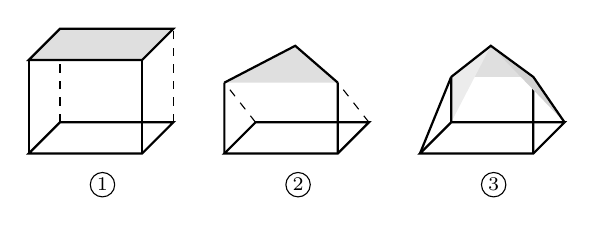
\begin{tikzpicture}[>=stealth, scale=0.72]
  \begin{scope}
    \coordinate (A) at (0,0);
    \coordinate (B) at (2.0,0);
    \coordinate (C) at (2.55,0.55);
    \coordinate (D) at (0.55,0.55);
    \coordinate (A1) at (0,1.65);
    \coordinate (B1) at (2.0,1.65);
    \coordinate (C1) at (2.55,2.2);
    \coordinate (D1) at (0.55,2.2);
    \draw[thick] (A)--(B)--(C)--(D)--cycle;
    \draw[thick] (A)--(A1) (B)--(B1);
    \draw[dashed] (C)--(C1) (D)--(D1);
    \fill[gray!25] (A1)--(B1)--(C1)--(D1)--cycle;
    \draw[thick] (A1)--(B1)--(C1)--(D1)--cycle;
    \node[circle,draw,inner sep=1pt] at (1.3,-0.55) {\scriptsize 1};
  \end{scope}
  \begin{scope}[xshift=3.45cm]
    \coordinate (A) at (0,0);
    \coordinate (B) at (2.0,0);
    \coordinate (C) at (2.55,0.55);
    \coordinate (D) at (0.55,0.55);
    \coordinate (M) at (1.25,1.9);
    \draw[thick] (A)--(B)--(C)--(D)--cycle;
    \draw[thick] (A)--(0,1.25) (B)--(2,1.25);
    \draw[dashed] (C)--(2,1.25) (D)--(0,1.25);
    \fill[gray!25] (0,1.25)--(M)--(2,1.25)--cycle;
    \draw[thick] (0,1.25)--(M)--(2,1.25);
    \node[circle,draw,inner sep=1pt] at (1.3,-0.55) {\scriptsize 2};
  \end{scope}
  \begin{scope}[xshift=6.9cm]
    \coordinate (A) at (0,0);
    \coordinate (B) at (2.0,0);
    \coordinate (C) at (2.55,0.55);
    \coordinate (D) at (0.55,0.55);
    \coordinate (M) at (1.25,1.9);
    \coordinate (L) at (0.55,1.35);
    \coordinate (R) at (2.0,1.35);
    \draw[thick] (A)--(B)--(C)--(D)--cycle;
    \draw[thick] (A)--(L) (B)--(R);
    \draw[dashed] (C)--(R) (D)--(L);
    \fill[gray!25] (L)--(M)--(R)--cycle;
    \fill[gray!15] (D)--(L)--(M)--cycle;
    \fill[gray!35] (M)--(R)--(C)--cycle;
    \draw[thick] (L)--(M)--(R) (D)--(L) (R)--(C);
    \node[circle,draw,inner sep=1pt] at (1.3,-0.55) {\scriptsize 3};
  \end{scope}
\end{tikzpicture}
\end{center}
\nopagebreak[4]
（A）$P_3>P_2>P_1$　　（B）$P_3>P_2=P_1$　　（C）$P_3=P_2>P_1$　　（D）$P_3=P_2=P_1$

\Needspace{0.4\textheight}
\end{question}
\begin{question}
\gkti{12}如图，小圆圈表示网络的结点，结点之间的连线表示它们有网线相联。连线标注的数字表示该段网线单位时间内可以通过的最大信息量。现从结点 $A$ 向结点 $B$ 传递信息，信息可以分开沿不同的路线同时传递，则单位时间内传递的最大信息量是\mbox{（　　）}
\nopagebreak[4]
\begin{center}% 2001 年全国新课程卷理科第 12 题：信息网络
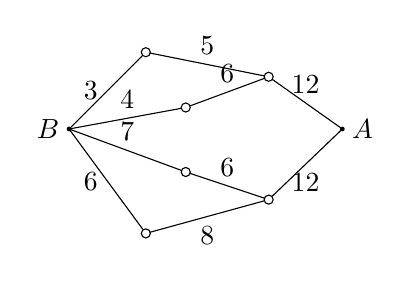
\begin{tikzpicture}[>=stealth, scale=0.78]
  \coordinate (B) at (0,0);
  \coordinate (U) at (1.25,1.25);
  \coordinate (V) at (3.25,0.85);
  \coordinate (M) at (1.9,0.35);
  \coordinate (N) at (1.9,-0.7);
  \coordinate (W) at (1.25,-1.7);
  \coordinate (Z) at (3.25,-1.15);
  \coordinate (A) at (4.45,0);

  \draw (B)--(U) node[midway, left] {3};
  \draw (U)--(V) node[midway, above] {5};
  \draw (B)--(M) node[midway, above] {4};
  \draw (M)--(V) node[midway, above] {6};
  \draw (B)--(N) node[midway, above] {7};
  \draw (N)--(Z) node[midway, above] {6};
  \draw (B)--(W) node[midway, left] {6};
  \draw (W)--(Z) node[midway, below] {8};
  \draw (V)--(A) node[midway, above] {12};
  \draw (Z)--(A) node[midway, below] {12};

  \foreach \point in {U,V,M,N,W,Z}
    \filldraw[fill=white] (\point) circle (2.1pt);
  \fill (B) circle (1.1pt) node[left] {$B$};
  \fill (A) circle (1.1pt) node[right] {$A$};
\end{tikzpicture}
\end{center}
\nopagebreak[4]
（A）$26$　　（B）$24$　　（C）$20$　　（D）$19$

\end{question}
\gkpart{二、填空题}

\begin{question}
\gkti{13}若复数 $z=\sqrt2+\sqrt6\,i$，则 $\arg\dfrac1z$ 等于\gkblank{}。

\end{question}
\begin{question}
\gkti{14}一个袋子里装有大小相同的 $3$ 个红球和 $2$ 个黄球。从中同时取出 $2$ 个，则其中含红球个数的数学期望是\gkblank{}。（用数字作答）

\end{question}
\begin{question}
\gkti{15}在空间中，①若四点不共面，则这四点中任何三点都不共线；②若两条直线没有公共点，则这两条直线是异面直线。以上两个命题中，逆命题为真命题的是\gkblank{}。（把符合要求的命题序号都填上）

\end{question}
\begin{question}
\gkti{16}设 $\{a_n\}$ 是公比为 $q$ 的等比数列，$S_n$ 是它的前 $n$ 项和。若 $\{S_n\}$ 是等差数列，则 $q=$\gkblank{}。

\end{question}
\gkpart{三、解答题}

\begin{question}
\gkti{17}解关于 $x$ 的不等式

\nopagebreak[4]
\[
\frac{x-a}{x-a^2}<0\qquad(a\in\mathbb R).
\]

\Needspace{0.4\textheight}
\end{question}
\begin{question}
\gkti{18}如图，用 $A$、$B$、$C$ 三类不同的元件连接成两个系统 $N_1$、$N_2$。当元件 $A$、$B$、$C$ 都正常工作时，系统 $N_1$ 正常工作；当元件 $A$ 正常工作且元件 $B$、$C$ 至少有一个正常工作时，系统 $N_2$ 正常工作。已知元件 $A$、$B$、$C$ 正常工作的概率依次为 $0.80,0.90,0.90$。
\nopagebreak[4]
\begin{center}% 2001 年全国新课程卷理科第 18 题：两个元件系统
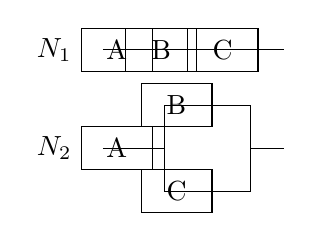
\begin{tikzpicture}[>=stealth, scale=0.78]
  \tikzset{component/.style={draw, rectangle, minimum width=0.9cm,
    minimum height=0.55cm, inner sep=1pt}}
  \node[left] at (0,1.45) {$N_1$};
  \draw (0.35,1.45)--(0.8,1.45)
    node[component, midway] {A}
    --(1.8,1.45)
    node[component, midway] {B}
    --(2.8,1.45)
    node[component, midway] {C}
    --(3.3,1.45);

  \node[left] at (0,-0.15) {$N_2$};
  \draw (0.35,-0.15)--(0.8,-0.15)
    node[component, midway] {A}
    --(1.35,-0.15);
  \draw (1.35,-0.15)--(1.35,0.55)--(1.75,0.55)
    node[component, midway] {B}
    --(2.75,0.55)--(2.75,-0.15);
  \draw (1.35,-0.15)--(1.35,-0.85)--(1.75,-0.85)
    node[component, midway] {C}
    --(2.75,-0.85)--(2.75,-0.15);
  \draw (2.75,-0.15)--(3.3,-0.15);
\end{tikzpicture}
\end{center}
\nopagebreak[4]
（1） 求系统 $N_1$ 正常工作的概率 $P_1$；

（2） 求系统 $N_2$ 正常工作的概率 $P_2$。

\end{question}
\begin{question}
\gkti{19}设 $a>0$，$f(x)=\dfrac{e^x}{a}+\dfrac{a}{e^x}$ 是 $\mathbb R$ 上的偶函数。

（1） 求 $a$ 的值；

（2） 证明 $f(x)$ 在 $(0,+\infty)$ 上是增函数。

\Needspace{0.4\textheight}
\end{question}
\begin{question}
\gkti{20}注意：考生在（20 甲）、（20 乙）两题中选一题作答，如果两题都答，只以（20 甲）计分。

【甲】如图，以正四棱锥 $V-ABCD$ 底面中心 $O$ 为坐标原点建立空间直角坐标系 $O-xyz$，其中 $Ox\parallel BC$，$Oy\parallel AB$。$E$ 为 $VC$ 中点，正四棱锥底面边长为 $2a$，高为 $h_0$。
\nopagebreak[4]
\begin{center}% 2001 年全国新课程卷理科第 20 题甲：正四棱锥坐标图
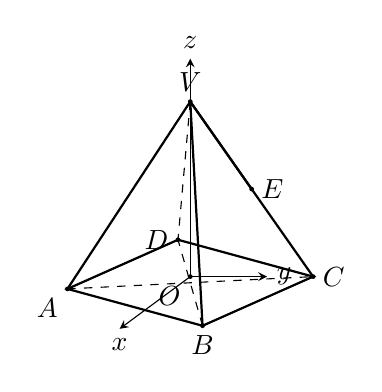
\begin{tikzpicture}[>=stealth, scale=0.78]
  \coordinate (A) at (-2.0,-0.4);
  \coordinate (B) at (0.2,-1.0);
  \coordinate (C) at (2.0,-0.2);
  \coordinate (D) at (-0.2,0.4);
  \coordinate (O) at (0, -0.2);
  \coordinate (V) at (0,2.65);
  \coordinate (E) at (1.0,1.225);

  \draw[thick] (A)--(B)--(C)--(D)--cycle;
  \draw[dashed] (A)--(C) (B)--(D);
  \draw[thick] (V)--(A) (V)--(B) (V)--(C);
  \draw[dashed] (V)--(D);
  \draw[thick] (V)--(E);
  \fill (A) circle (1.1pt) node[below left] {$A$};
  \fill (B) circle (1.1pt) node[below] {$B$};
  \fill (C) circle (1.1pt) node[right] {$C$};
  \fill (D) circle (1.1pt) node[left] {$D$};
  \fill (O) circle (1.1pt) node[below left] {$O$};
  \fill (V) circle (1.1pt) node[above] {$V$};
  \fill (E) circle (1.1pt) node[right] {$E$};
  \draw[->] (O)--(-1.15,-1.05) node[below] {$x$};
  \draw[->] (O)--(1.25,-0.2) node[right] {$y$};
  \draw[->] (O)--(0,3.35) node[above] {$z$};
\end{tikzpicture}
\end{center}
\nopagebreak[4]
（1） 求 $\cos\langle\overrightarrow{BE},\overrightarrow{DE}\rangle$；

（2） 记面 $BCV$ 为 $\alpha$，面 $DCV$ 为 $\beta$，若 $\angle BED$ 是二面角 $\alpha-VC-\beta$ 的平面角，求 $\angle BED$。

【乙】如图，在底面是直角梯形的四棱锥 $S-ABCD$ 中，$\angle ABC=90^\circ$，$SA\perp$ 面 $ABCD$，$SA=AB=BC=1$，$AD=\dfrac12$。
\nopagebreak[4]
\begin{center}% 2001 年全国新课程卷理科第 20 题乙：直角梯形底面的四棱锥
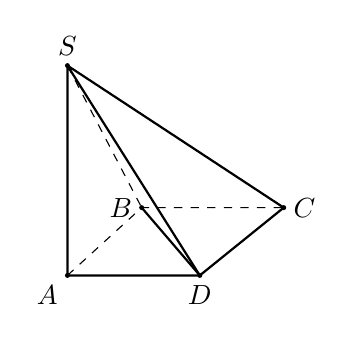
\begin{tikzpicture}[>=stealth, scale=0.82]
  \coordinate (A) at (0,0);
  \coordinate (B) at (1.15,1.05);
  \coordinate (C) at (3.35,1.05);
  \coordinate (D) at (2.05,0);
  \coordinate (S) at (0,3.25);

  \draw[thick] (S)--(A) (S)--(C) (S)--(D);
  \draw[dashed] (S)--(B);
  \draw[thick] (A)--(D)--(C);
  \draw[dashed] (A)--(B)--(C);
  \draw[thick] (B)--(D);

  \fill (S) circle (1.1pt) node[above] {$S$};
  \fill (A) circle (1.1pt) node[below left] {$A$};
  \fill (B) circle (1.1pt) node[left] {$B$};
  \fill (C) circle (1.1pt) node[right] {$C$};
  \fill (D) circle (1.1pt) node[below] {$D$};
\end{tikzpicture}
\end{center}
\nopagebreak[4]
（1） 求四棱锥 $S-ABCD$ 的体积；

（2） 求面 $SCD$ 与面 $SBA$ 所成的二面角的正切值。

\Needspace{0.4\textheight}
\end{question}
\begin{question}
\gkti{21}某电厂冷却塔的外形是如图所示双曲线的一部分绕其中轴（即双曲线的虚轴）旋转所成的曲面，其中 $A,A'$ 是双曲线的顶点，$C,C'$ 是冷却塔上口直径的两个端点，$B,B'$ 是下底直径的两个端点，已知 $AA'=14\ \mathrm m$，$CC'=18\ \mathrm m$，$BB'=22\ \mathrm m$，塔高 $20\ \mathrm m$。

（1） 建立坐标系并写出该双曲线方程；

（2） 求冷却塔的容积（精确到 $10\ \mathrm m^3$，塔壁厚度不计，$\pi$ 取 $3.14$）。
\nopagebreak[4]
\begin{center}% 2001 年全国新课程卷理科第 21 题：冷却塔双曲线截面
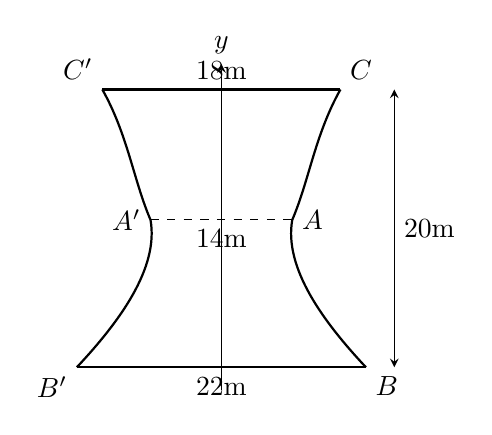
\begin{tikzpicture}[>=stealth, scale=0.72]
  \coordinate (TL) at (-2.1,2.45);
  \coordinate (TR) at (2.1,2.45);
  \coordinate (ML) at (-1.25,0.15);
  \coordinate (MR) at (1.25,0.15);
  \coordinate (BL) at (-2.55,-2.45);
  \coordinate (BR) at (2.55,-2.45);

  \draw[thick] (TL) .. controls (-1.65,1.65) and (-1.55,0.85) .. (ML)
    .. controls (-1.1,-0.7) and (-1.8,-1.65) .. (BL);
  \draw[thick] (TR) .. controls (1.65,1.65) and (1.55,0.85) .. (MR)
    .. controls (1.1,-0.7) and (1.8,-1.65) .. (BR);
  \draw[thick] (TL)--(TR) node[midway, above] {$18\mathrm{m}$};
  \draw[thick] (BL)--(BR) node[midway, below] {$22\mathrm{m}$};
  \draw[dashed] (ML)--(MR) node[midway, below] {$14\mathrm{m}$};
  \draw[<->] (3.05,-2.45)--(3.05,2.45) node[midway, right] {$20\mathrm{m}$};
  \draw[->] (0,-2.85)--(0,2.9) node[above] {$y$};
  \node[above left] at (TL) {$C'$};
  \node[above right] at (TR) {$C$};
  \node[left] at (ML) {$A'$};
  \node[right] at (MR) {$A$};
  \node[below left] at (BL) {$B'$};
  \node[below right] at (BR) {$B$};
\end{tikzpicture}
\end{center}
\nopagebreak[4]
\end{question}
\begin{question}
\gkti{22}设 $0<\theta<\dfrac\pi2$，曲线

\nopagebreak[4]
\[
x^2\sin\theta+y^2\cos\theta=1
\]

\Needspace{5\baselineskip}
和

\nopagebreak[4]
\[
x^2\cos\theta-y^2\sin\theta=1
\]

有 $4$ 个不同的交点。

（1） 求 $\theta$ 的取值范围；

（2） 证明这 $4$ 个交点共圆，并求圆半径的取值范围。

\end{question}